\documentclass[12pt]{report}
\usepackage{amsmath,amsthm,amssymb,amsfonts,setspace,graphicx,subfigure,verbatim}
\usepackage{adjustbox}

\usepackage{listings}
\usepackage[italian]{babel}
\usepackage[a4paper, portrait, margin=0.85in]{geometry}

\usepackage[colorlinks]{hyperref}

\lstdefinelanguage{AMPL}{keywords={set,param,var,arc,integer,minimize,maximize,subject,to,node,sum,in,Current,complements,integer,solve_result_num,IN,contains,less,suffix,INOUT,default,logical,sum,Infinity,dimen,max,symbolic
,Initial,div,min,table,LOCAL,else,option,then,OUT,environ,setof ,union,all,exists,shell_exitcodeuntil,binary,forall,solve_exitcodewhile ,by,if,solve_messagewithin,check,in,solve_result
},sensitive=true,comment=[l]{\#}}

\lstset{frame=tb,
  language=AMPL,
  aboveskip=3mm,
  belowskip=3mm,
  showstringspaces=false,
  columns=flexible,
  basicstyle={\ttfamily},
  numbers=none,
  numberstyle=\tiny\color{gray},
  keywordstyle=\bfseries,
  commentstyle=\textit,
  stringstyle=\color{mauve},
  breaklines=true,
  breakatwhitespace=true,
  tabsize=3
}



\begin{document}
\title{Ricerca operativa}
\author{Ollari Ischimji Dmitri}

\maketitle

\newpage

\tableofcontents
\listoffigures
\listoftables

% TODO: arrivato a pagina 45
\chapter{Modelli}
\section{Flusso a costo minimo}


Tipico problema di calcolo computazionale che ha le seguenti caratteristiche per i nodi:
\begin{itemize}
	\item \textbf{Nodi sorgente}: nodi che producono il flusso
	\item \textbf{Nodi destinazione}: nodi che consumano il flusso
	\item \textbf{Nodi transito}: nodi che non sono né sorgenti né destinazioni
\end{itemize}

Per ogni arco $(i, j) \in A$ sono associati dei costi unitari $c_{ij}$ per unità di flusso che si spostano da $i$ a $j$, è
possibile la presenza di $d_{ij}$ che indica la capacità massima dell'arco $(i, j)$.

Il prodotto \textit{trasmesso} lungo un'arco del grafo è il flusso $x_{ij}$, che deve essere minore o uguale alla capacità
ma non negativo.

Per calcolare il flusso uscente dal nodo $i$:
\begin{align}
	\sum_{j: (i, j) \in A} x_{ij}
\end{align}

Mentre il flusso uscente dal nodo $i$:
\begin{align}
	\sum_{j: (j, i) \in A} x_{ji}
\end{align}

I vincoli del problema derivanti dalla conservazione del flusso sono:
\begin{align}
	\sum_{j: (i, j) \in A} x_{ij} - \sum_{j: (j, i) \in A} x_{ji} = b_i \quad \forall i \in V
\end{align}



Il modello matematico completo è:
\begin{align}
	 & \min \sum_{(i, j) \in A} c_{ij} x_{ij}                                                    \\
	 & \sum_{j: (i, j) \in A} x_{ij} - \sum_{j: (j, i) \in A} x_{ji} = b_i \quad \forall i \in V \\
	 & 0 \leq x_{ij} \leq d_{ij} \quad \text{interi} \quad \forall (i, j) \in A
	\label{eq:flusso_costo_minimo}
\end{align}

\subsection{Matrice dei vincoli}

La matrice cha ha tante \textbf{righe} quanti sono i \textbf{vincoli} e tante \textbf{colonne}
quante sono le \textbf{variabili}.

La matrice dei vincoli di uguaglianza per i problemi di flusso a costo minimo coincide
con la matrice di incidenza \textbf{nodo-arco} della rete.

\subsection{Esempio}
\begin{figure}[!ht]
	\centering
	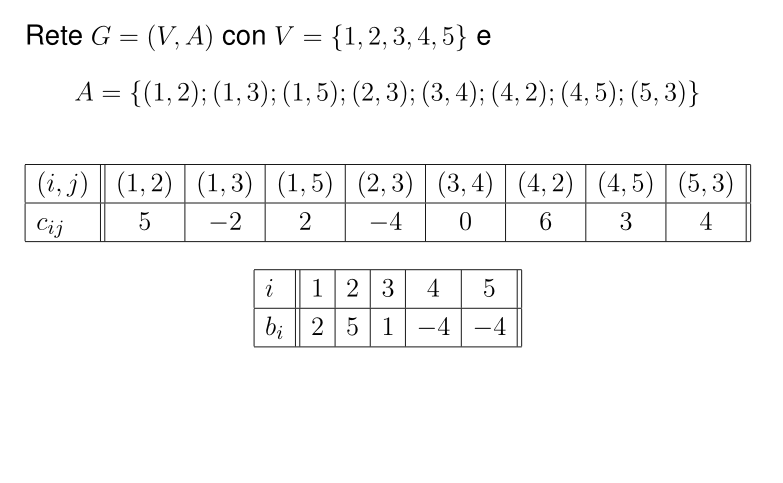
\includegraphics[scale=0.4]{./images/matrice_vincoli.png}
	\label{fig:matrice_vincoli}
	\caption{Matrice dei vincoli}
\end{figure}

Il modello matematico dell'esempio è:
\begin{align}
	 & \min 5x_{12} - 4x_{23} + 6x_{42} - 2x_{13} + 0x_{34} + 3x_{15} + 4x_{53} + 3x_{45} \\
	 & x_{12} + x_{13} + x_{15} = 2                                                       \\
	 & x_{23} - x_{12} - x_{42} = 5                                                       \\
	 & x_{34} - x_{13} - x_{23} - x_{53} = 1                                              \\
	 & x_{42} + x_{45} - x_{34} = -4                                                      \\
	 & x_{53} + x_{15} - x_{45} = -4                                                      \\
	 & x_{ij} \geq 0 \quad \forall (i, j) \in A
\end{align}

La matrice dei vincoli è:
\begin{table}
	\begin{adjustbox}{width=0.4\columnwidth,center}
		\begin{tabular}{|c|c|c|c|c|c|c|c|c|}
			\hline
			  & $x_{12}$ & $x_{13}$ & $x_{15}$ & $x_{23}$ & $x_{42}$ & $x_{34}$ & $x_{53}$ & $x_{45}$ \\
			\hline
			1 & 1        & 1        & 1        & 0        & 0        & 0        & 0        & 0        \\
			2 & -1       & 0        & 0        & 1        & -1       & 0        & 0        & 0        \\
			3 & 0        & -1       & 0        & -1       & 0        & 1        & -1       & 0        \\
			4 & 0        & 0        & 0        & 0        & 0        & -1       & 0        & 1        \\
			5 & 0        & 0        & -1       & 0        & 0        & 0        & 0        & -1       \\
			\hline
		\end{tabular}
	\end{adjustbox}
\end{table}

Il modello matematico per la risoluzione scritto in \textbf{ampl} è:

\begin{adjustbox}{width=0.8\columnwidth,center}
	\begin{lstlisting}{AMPL}
### INSIEMI ###
  set NODI ;
  set ARCHI within NODI cross NODI ;
### PARAMETRI ###
  param b{NODI};
  param c{ARCHI} ;
  param d{ARCHI} >= 0, default Infinity ;
### VARIABILI ###
  var x{(i, j) in ARCHI} >= 0, <= d[i,j], integer ;
### VINCOLI ###
  subject to bilancio{i in NODI} : sum{j in NODI : (i, j) in ARCHI} x[i,j] - sum{j in NODI :
  (j, i) in ARCHI} x[j,i] = b[i] ;
### OBIETTIVO ###
  minimize costo_totale : sum{(i, j) in ARCHI} c[i,j]*x[i,j] ;
  \end{lstlisting}
\end{adjustbox}


I dati del problema sono:

\begin{adjustbox}{width=0.8\columnwidth,center}
	\begin{lstlisting}{AMPL}
### INSIEMI ###
    set NODI := n1 n2 n3 n4 n5 ;
    set ARCHI := (n1,n2) (n1,n3) (n1,n5) (n2,n3) (n3,n4) (n4,n2) (n4,n5) (n5,n3) ;
### PARAMETRI ###
    param b :=
    n1 2
    n2 5
    n3 1
    n4 -4
    n5 -4 ;

    param c :=
    n1 n2 5
    n1 n3 -2
    n1 n5 2
    n2 n3 -4
    n3 n4 0
    n4 n2 6
    n4 n5 3
    n5 n3 4 ;
  \end{lstlisting}
\end{adjustbox}




\section{Flusso massimo}

Simile al problema di flusso a costo minimo, ma senza i costi unitari $c_{ij}$,
quindi si vuole massimizzare il flusso che attraversa la rete.

\subsection{Modello matematico}
Le variabili del modello matematico per questo problema sono:
\begin{itemize}
	\item $x_{ij} \geq 0$: flusso lungo l'arco $(i, j)$
	\item $d_{ij}$: capacità massima dell'arco $(i, j)$
	\item $x_{ij} \leq d_{ij} \quad \forall (i, j) \in A$
	\item $\sum_{j: (i, j) \in A} x_{ij} = \sum_{j: (j, i) \in A} x_{ji} \quad \forall i \in V \backslash \{S, D\}$ equivalente a dire che il flusso entrante in un nodo è uguale al flusso uscente dal nodo
\end{itemize}


L'obiettivo del problema è quello di massimizzare la quantità di flusso che esce dal nodo sorgente $S$:
\begin{align}
	\sum_{j: (S, j) \in A} x_{Sj}
\end{align}

Che corrisponde al'aumentare il flusso del nodo destinazione $D$:
\begin{align}
	\sum_{j: (j, D) \in A} x_{jD}
\end{align}


Il modello matermatico completo è:
\begin{align}
	 & \max \sum_{j: (S, j) \in A} x_{Sj}                                                                      \\
	 & \sum_{j: (i, j) \in A} x_{ij} = \sum_{j: (j, i) \in A} x_{ji} \quad \forall i \in V \backslash \{S, D\} \\
	 & 0 \leq x_{ij} \leq d_{ij} \quad \forall (i, j) \in A
\end{align}

\textbf{OSS}: La matrice dei vincoli di uguaglianza del problema di flusso massimo coincide
con la matrice di incidenza node-arco della rete senza i nodi sorgente e destinazione.



\subsection{Esempio}
La rete ha le seguenti caratteristiche:

\begin{table}[!ht]
	\begin{adjustbox}{width=0.4\columnwidth,center}
		\begin{tabular}{|c|c|c|c|c|c|c|c|c|}
			\hline
			Arco     & $(S, 1)$ & $(S, 2)$ & $(1, 3)$ & $(1, 4)$ & $(2, 3)$ & $(2, 1)$ & $(3, D)$ & $(4, D)$ \\
			\hline
			Capacità & 3        & 2        & 1        & 4        & 1        & 1        & 1        & 7        \\
			\hline
		\end{tabular}
	\end{adjustbox}
\end{table}


Il modello matematico per l'esempio è:

\begin{align}
	 & \max x_{S1} + x_{S2}                                         \\
	 & x_{13} + x_{14} - x_{S1} = 0                                 \\
	 & x_{23} + x_{24} - x_{S2} = 0                                 \\
	 & x_{3D} - x_{13} - x_{23} = 0                                 \\
	 & x_{4D} - x_{14} - x_{24} = 0                                 \\
	 & 0 \leq x_{S1} \leq 3                                         \\
	 & 0 \leq x_{S2} \leq 2                                         \\
	 & 0 \leq x_{13} \leq 1                                         \\
	 & 0 \leq x_{14} \leq 4                                         \\
	 & 0 \leq x_{23} \leq 1                                         \\
	 & 0 \leq x_{24} \leq 1                                         \\
	 & 0 \leq x_{3D} \leq 1                                         \\
	 & 0 \leq x_{4D} \leq 7                                         \\
	 & x_{ij} \geq 0 \quad \text{interi} \quad \forall (i, j) \in A
\end{align}

La matrice dei vincoli che ne consegue è:
\begin{table}[!ht]
	\begin{adjustbox}{width=0.4\columnwidth, center}
    \begin{tabular}{|c|c|c|c|c|c|c|c|c|}
      \hline
      & $x_{S1}$ & $x_{S2}$ & $x_{13}$ & $x_{14}$ & $x_{23}$ & $x_{24}$ & $x_{3D}$ & $x_{4D}$ \\
      \hline
      1 & -1       & 0        & 1        & 1        & 0        & 0        & 0        & 0        \\
      2 & 0        & -1       & 0        & 0        & 1        & 1        & 0        & 0        \\
      3 & 0        & 0        & -1       & 0        & -1       & 0        & 1        & 0        \\
      4 & 0        & 0        & 0        & -1       & 0        & -1       & 0        & 1        \\
      \hline
    \end{tabular}
	\end{adjustbox}
\end{table}

Il modello matematico per la risoluzione scritto in \textbf{ampl} è:
\begin{lstlisting}{AMPL}
### INSIEMI ###
    set NODI ;
    set ARCHI within NODI cross NODI ;
### PARAMETRI ###
    param Sorgente symbolic in {NODI};
    param Destinazione symbolic in {NODI} , != Sorgente ;
    param d{ARCHI} >= 0, default Infinity ;
### VARIABILI ###
    var x{(i, j) in ARCHI} >= 0, <= d[i,j], integer ;
### VINCOLI ###
    subject to equilibrio{i in NODI diff {Sorgente, Destinazione}} : sum{j in NODI : (i, j) in
    ARCHI} x[i,j] - sum{j in NODI : (j, i) in ARCHI} x[j,i] = 0 ;
### OBIETTIVO ###
    maximize flusso_uscente : sum{j in NODI : (Sorgente,j) in ARCHI} x[Sorgente,j] ;
\end{lstlisting}




% WARN: partito da pdf nuovo, riguardare i pdf delle lezioni precedenti
% TODO: arrivato a pagina 29
%
\chapter{Teoria della programmazione lineare}

I problemi di programmazione lineare(PL) in forma scalare canonica sono sempre problemi di massimo con vincoli di minore uguale e con vincoli non negativi.

In forma scalare i problemi di programmazione lineare sono espressi come:
\begin{align}
	 & \max \sum_{j=1}^n c_j x_j                              \\
	 & \sum_{j=1}^n a_{ij} x_j \leq b_i \quad i = 1, \dots, m \\
	 & x_j \geq 0 \quad j =1, \dots, n
\end{align}

Mediante l'uso dei \textbf{vettori} osservo che:
\begin{align}
	cx = \sum_{j=1}^n c_j x_j \\
\end{align}
\begin{align}
	a_i x = \sum_{j=1}^n a_{ij} x_j
\end{align}

In questo modo posso riscrivere il problema di programmazione lineare come:
\begin{align}
	 & \max cx                              \\
	 & a_i x \leq b_i \quad i = 1, \dots, m \\
	 & x \geq
\end{align}

Anche le matrici vengono in aiuto, considerando una matrice $A \in \mathbb{R}^{m\times n}$ che ha tante \textbf{righe} quanti i vincoli (m) e la ci $i$-esima riga è il vettore $a_i$.

Si considera anche il vettore $b=(b_1, \dots, b_m) \in \mathbb{R}^{m}$ di dimensione $m$ che contiene i termini noti dei vincoli.

Nota che $Ax = (a_1 x, \dots, a_m x)$, la reppresentazione \textbf{matriciale} è :
\begin{align}
	 & \max cx   \\
	 & Ax \leq b \\
	 & x \geq 0
\end{align}


\section{PL canonici $\equiv$ PL generici}

\subsection{Trasformazione da $\min$ a $\max$}

\begin{align}
	\min cx \equiv - \max -cx
\end{align}

\subsection{Trasformazione da $\geq$ a $\leq$}

\begin{align}
	a_i x \geq b_i \equiv -a_i x \leq -b_i
\end{align}

\subsection{Trasformazione da $=$ a $\leq$}

\begin{align}
	a_i x = b_i \equiv \begin{cases}
		                   a_i x \leq b_i \\
		                   -a_i x \leq -b_i
	                   \end{cases}
\end{align}


\subsection{Sostituzione variabili $\leq 0$ con variabili $\geq 0$}

Data una variabile $x_j \leq 0$ si sostituisce con $x_j = -x_j'$ dove $x_j' \geq 0$.


\subsection{Sostituzione variabili libere con differenza di variabili $\geq 0$}

Avendo una variabile $x_j$ libera si sostituisce con $x_j' - x_j''$ con $x_j', x_j'' \geq 0$.


\section{Insiemi}
\subsection{Insieme convesso}

Un'insieme $C \subseteq \mathbb{R}^n$ è convesso se:
\begin{align}
	\forall x_1, x_2 \in C, \quad \forall \lambda \in [0,1] : \quad \lambda x_1 + (1-\lambda) x_2 \in C
\end{align}

Il segmento che unisce i due punti fa parte dell'insieme.

\subsection{insiemi limitati e chiusi}

Un'insieme $C$ è limitato se esiste una sfera di raggio finito che contiene $C$.


Un'insieme $C$ è chiuso se contiene tutti i suoi punti di frontiera.

\subsection{Semispazio e iperpiano}

Si definisce semispazio in $\mathbb{R}^n$ l'insieme di punti che soddisfano una disequazione lineare del tipo:
\begin{align}
	\sum_{j=1}^n w_j x_j \leq v
\end{align}

In forma vettoriale posso riscrivere come:
\begin{align}
	wx \leq v
\end{align}


Si definisce iperpiano in $\mathbb{R}^n$ l'insieme di punti che soddisfano una disequazione lineare del tipo:
\begin{align}
	\sum_{j=1}^n w_j x_j = v
\end{align}

In forma vettoriale posso riscrivere come:
\begin{align}
	wx = v
\end{align}


\subsection{Poliedro e politopo}

Si definisce poliedro l'insieme di un numero finito di semispazi e/o iperpiani, se il poliedro è limitato, l'intersezione prende il nome di politopo(letto come politopò e non politòpo).



\section{Regione ammissibile}

La regione ammissibile $S_a$ di un problema di PL in forma canonica è un poliedro:
\begin{align}
	S_a = \{x \in \mathbb{R}^n : a_i x \leq b_i,  i = 1, \dots, m, x \geq 0 \}
\end{align}


Si noti che:
\begin{itemize}
	\item I sempispazi e iperspazi sono insiemi chiusi
	\item L'intersezione di insiemi chiusi è un insieme chiuso
\end{itemize}

I poliedri sono insiemi chiusi, quindi anche la regione ammissibile $S_a$ è un'insieme chiuso.


\subsection{Convessità}

Siano $x, y \in S_a$:
\begin{align}
	a_i x \leq b_i,  i = 1, \dots, m, x \geq 0 \\
	a_i y \leq b_i,  i = 1, \dots, m, y \geq 0
\end{align}


Quindi $\forall \lambda \in (0,1)$ e $\forall i = 1, \dots, m$:
\begin{align}
	a_i [\lambda x + (1-\lambda) y] & =                               \\
	                                & = \lambda b_i + (1-\lambda) b_i \\
	                                & = b_i
\end{align}



Inoltre:
\begin{align}
	\lambda x + (1-\lambda) y \in S_a
\end{align}

Che ci fa capire che $S_a$ è convesso.


\subsection{Limitatezza e illimitatezza}


La regione ammissibile Sa di un problema di PL è un poliedro e come tale è un insieme chiuso e convesso. Inoltre, può essere un insieme vuoto, un insieme limitato (politopo) oppure un insieme illimitato.


\section{Vertici della regione ammissibile}

Si definisce vertice di $S_a$ un punto $\bar{x} \in S_a$ tale che $\nexists x_1, x_2 \in S_a, x \neq x_2$ tali che:
\begin{align}
  \bar{x} = 0.5 x_1 + 0.5 x_2
\end{align}

Ovvero $\bar{x}$ è il punto medio del segmento che unisce $x_1$ e $x_2$.



Ne derica che se un problema di programmazione in forma canonica ha $S_a\neq \emptyset$, allora ha almeno un vertice.


\section{Raggi}

ARRIVATO A PAGINA 29


\end{document}

